% DO NOT COMPILE THIS FILE DIRECTLY!
% This is included by the other .tex files.

\begin{frame}[t,plain]
\titlepage
\end{frame}

\begin{frame}
	\frametitle{Plan for this session}
	\begin{itemize}
            \item Review the following:
            \begin{itemize}
		\item The layout of the codebase
                \item Some design principles
                \item Architecture of the application
            \end{itemize}
            \item Generally anything that might be relevant when reviewing the codebase
	\end{itemize}
\end{frame}

\begin{frame}
	\frametitle{The software stack}
	\begin{itemize}
                \item CakePHP 4.x
                \item Bootstrap 4 UI
                \item A host of ported and modernesied MISP libraries
                \item Database: MySQL / raw file storage
                \item Redis will be added in the future
	\end{itemize}
\end{frame}

\begin{frame}
	\frametitle{Basic design principles}
	\begin{itemize}
		\item MVC design
                \item API / UI dual design
                \item ReSTful APIs
                \item Heavy on abstraction
	\end{itemize}
\end{frame}

\begin{frame}
\frametitle{Basic design principles - UI}
\begin{center}
    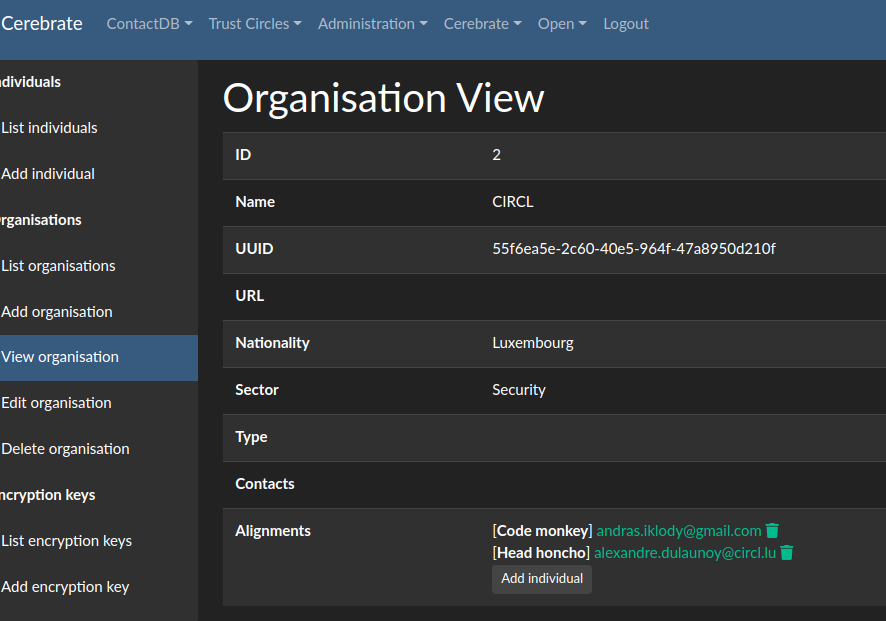
\includegraphics[scale=0.5]{UI.png}
\end{center}
\end{frame}

\begin{frame}
\frametitle{Basic design principles - API}
\begin{center}
    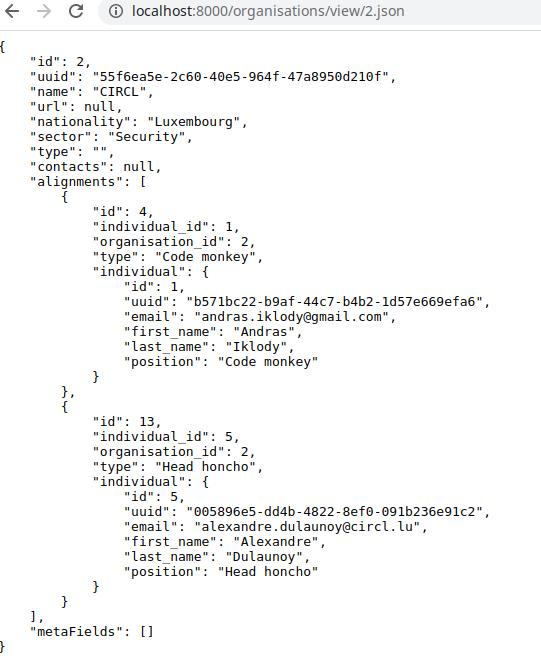
\includegraphics[scale=0.5]{API.png}
\end{center}
\end{frame}

\begin{frame}
	\frametitle{Directory structure}
	\begin{itemize}
            \item src
            \begin{itemize}
                \item Command
                \item Controller
                \item Model
                \item View
            \end{itemize}
            \item templates
            \item libraries
	\end{itemize}
\end{frame}

\begin{frame}
	\frametitle{Controllers}
	\begin{itemize}
            \item Inheritance of the AppController
            \item Reusable code via components
            \begin{itemize}
                \item CRUDComponent
                \item ACLComponent
                \item ParamHandlerComponent
                \item RestResponse Component
            \end{itemize}
	\end{itemize}
\end{frame}

\begin{frame}
	\frametitle{Controllers}
	\begin{itemize}
            \item Generally access public functions by /controller/action
            \item Response is always split between two paths: UI/API
            \item We can therefore test all functionalities via the API, the UI uses the same program logic
	\end{itemize}
\end{frame}


\begin{frame}
	\frametitle{Models}
	\begin{itemize}
		\item Tables
                \item Entities
                \item Tables Implement AppTable
                \item Entities implement AppModel
                \item Reusable code: Behaviors
	\end{itemize}
\end{frame}

\begin{frame}
	\frametitle{View layer}
	\begin{itemize}
		\item Reusable code in Views
                \item Templates
                \begin{itemize}
                    \item UI factories for change management and unifority
                    \item Parametrised view templating
                \end{itemize}
                \item Exception: API does not use views, rather serializes response data in the controller
	\end{itemize}
\end{frame}

\begin{frame}
	\frametitle{CLI tools}
	\begin{itemize}
		\item The plan is to feature a wide range of tools for the CLI
                \item Currently it's only in use for one use-case (password resets)
                \item CLI commands directly interact with the model, no controller code is executed
	\end{itemize}
\end{frame}

\begin{frame}
\frametitle{CLI tools}
\begin{center}
    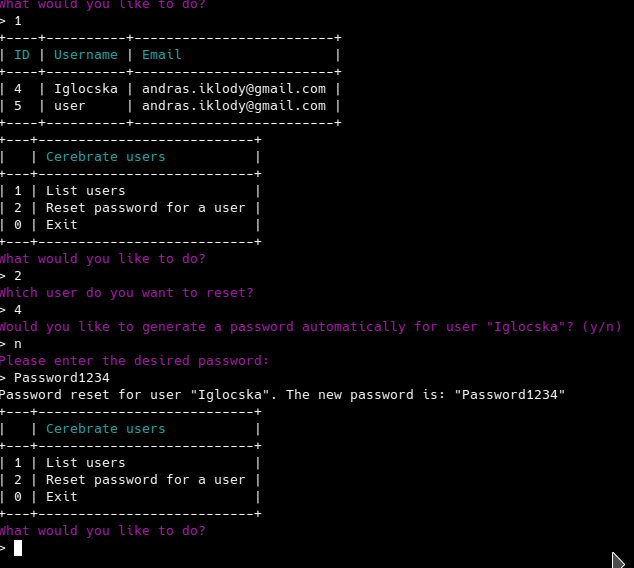
\includegraphics[scale=0.5]{CLI.png}
\end{center}
\end{frame}

\begin{frame}
	\frametitle{Authentication and RBAC}
	\begin{itemize}
            \item Authentication
            \begin{itemize}
		\item Username / API key
                \item Will be extended in the future, pending also requirement collection
            \end{itemize}
            \item RBAC
            \begin{itemize}
		\item Users are tied to role objects
                \item Roles are modifiable permission control tables
                \item The ACL component uses the user session's role to determine access for the requested endpoint
                \item We deny by default
            \end{itemize}
	\end{itemize}
\end{frame}

\begin{frame}
\frametitle{Authentication and RBAC}
\begin{center}
    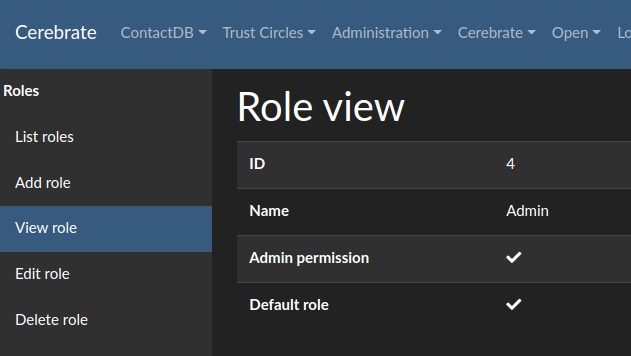
\includegraphics[scale=0.5]{roles.png}
\end{center}
\end{frame}

\begin{frame}
	\frametitle{Open directoy feature}
	\begin{itemize}
		\item Currently in early stages
                \item Opt-in system to publicly disclose organisation lists (act as a public trust authority)
                \item Unauthenticated endpoints, controlled by the configuration file
	\end{itemize}
\end{frame}

\begin{frame}
	\frametitle{JSON vocabularies}
	\begin{itemize}
		\item Potential point to test: JSON libraries ingested by Cerebrate
                \item Currently one use-case - extending models with meta fields
	\end{itemize}
\end{frame}

\begin{frame}
	\frametitle{Plans for the future in terms of major subsystems}
	\begin{itemize}
		\item Cerebrate to Cerebrate exchange, similar to the MISP synchronisation
                \item Cerebrate to local tool exchange using a modular approach
                \item Trust relationships with a direct ingestion and inbox system tier
	\end{itemize}
\end{frame}

